\chapter{Heat shield}
\qquad A complete deorbiting mission from LEO to GEO and returning to LEO has a very high delta-V requirement of  roughly $8.5$ km/s. To reduce this delta-V the GREDER spacecraft will use atmospheric drag in the upper atmosphere at an altitude of $70-120$ km to reduce its relative velocity when returning from GEO to LEO. This kind of maneuver is called an aerobrake and has the potential to save a significant amount of fuel and total spacecraft mass. Aerobrakes are commonly used for reentry vehicles. However, these experience very high thermal loads since the kinetic energy is converted to heat through friction with the atmosphere in a single reentry trajectory. Thus, a high mass for a heat shield is necessary. For a reusable spacecraft ablative heat shields are not useful. Instead, a passively cooled thermal protection system (TPS) was chosen. This allows to radiate the heat away. When the velocity is reduced into small increments the spacecraft can radiate the heat away in the time between the aerobrakes. The advantage is, that fuel is only required for trimming maneuvers to set the targeted perigee radius and not for the decelleration itself. A high number of aerobrakes can be performed with relatively small heat loads if extended mission time is not of a large concern.\\

Since the GREDER spacecraft is unmanned and does not utilize cryogenic fuels the extended mission time is not as critical. A heat shield needs to be developed for the spacecraft to protect it at the areas with the highest heat loads.\\

For first rough calculations the total velocity reduced by the aerobrakes was determined as $2.4$ km/s. This is the difference in velocity between the perigee velocity of the transfer orbit from GEO to aerobraking altitude and the velocity of the perigee of the transfer orbit from the last aerobrake to LEO. The mass of the spacecraft after deorbiting was estimated at $3500$ kg. This results in a kinetic energy of:

\begin{equation}
	E_{kinetic} = \frac{m_{sc}\Delta v^2}{2} = 10.04\ GJ
\end{equation}

For a number of $15$ aerobrakes this kinetic energy needs to be divided by $15$ assuming the temperature at the beginning of each aerobrake will be the same.  This kinetic energy was then assumed to be completely converted to thermal energy and distributed evenly over the mass of a heat shield. With the maximum allowable temperature of the chosen material a rough required heat shield mass could be estimated.
\begin{align}
	E_{kinetic} &= \frac{mv^2}{2}\\
	m_{shield} &=\frac{E_{kinetic}}{c\times dT}
\end{align}
\begin{table}
	\centering
	\footnotesize
	\begin{tabular}{|c|c|c|c|c|}
		\hline
		Property & \makecell{Reinforced\\ Carbon-Carbon} & \makecell{Aluminium\\ (2024-T8XX)} & \makecell{Steel\\ Type 321} & \makecell{Titanium (6A1-4V)}\\
		\hline
		Density (kg/m$^3$) & $1578$ & $2803$ & $8027$ & $4437$\\
		\hline
		\makecell{Thermal conductivity\\ ($W/m-K$)} & $3.9^*$ & $145.4$ & $14.7$ & $69$\\
		\hline 
		\makecell{Specific heat\\ ($J/kg-K$)} & $711.8$ & $816.4$ & $565.2$ & $523.4$\\
		\hline 
		\makecell{Multipule Use\\ Temperature Limit ($K$)} & $1922$ & $ 425^{**}$ & $872^{**}$ & $662^{ **}$\\
		\hline 
		\makecell{Single Use\\ Temperature Limit ($K$)} & $2033$ & $450$ & $922$ & $700$\\
		\hline
		$T_{cond}\times M_{TempLim} (E+6)$ & $1.41$ & $0.35$ & $0.49$ & $0.35$\\
		\hline 

	\end{tabular}
\vspace*{0.2cm}
 (*thru-the-thickness not isotropic; **values extrapolated by ratio of single/multiple use of CFRC) 
	\caption{Comparison of materials for heat shield}
\end{table}
The table above is a comparison of possible TPS materials. The values are taken from the TPSX NASA Material Properties Database. Multiple Use Temperature values were not available for the chosen metals but were extrapolated based on the ratio of the multiple and single use temperature limits of CFRC. The last row shows the product of the values of the lines Specific Heat and Multiple Use Temperature Limit. This relative value allows to quickly compare the materials with euach other regarding the required mass for a heat shield. The unit is J/kg showing that a high value is favorable to store as much energy as possible per mass.\\

Carbon Fibre Reinforced Carbon quickly proves as the material of choice for a low heat shield mass. Several metals were also taken into account since the manufacturing and integration into the spacecraft struture would be a lot easier. But the low mass for a CFRC TPS in combination with the low thermal conductivity made this the material of choice. CFRC was utilised in the space shuttle heat shield and was found to be the cause of the columbia catastrophe since it is quite brittle and thus sensitive to impact (Columbia Accident Investigation Board Report \footnote{\url{https://www.nasa.gov/columbia/home/CAIB\_Vol1.html}}). But since the GREDER spacecraft will be launched inside a rocket launcher fairing no high velocity impacts are to be expected. The capturing of the satellite on the nose cone will be done at very low relative velocities since the force applied by the magnets is controllable with the applied current and can be carefully adjusted (compare \autoref{sec:5}).
\begin{equation}
	m_{shield_{cc}}= \frac{m_{sc} \times (\Delta v_5\times 1000)^2}{2n_{ab}c_{cc}(T_{max_{cc}}-T_0)}
\end{equation}

With :
\begin{itemize}
	\item $\Delta v_5$ : Required $\Delta v$
	\item $m_{sc}$ : Spacecraft mass
	\item $n_{ab}$ : Number of aerobrakes
	\item $T_{max}$ : Maximum allowable temperature of CFRC
	\item $T_0$ : Temperature at beginning of aerobrakes
\end{itemize}

An aerobrake can also be used to change the inclination of the orbital plane. To achieve this the spacecraft needs to be a lifting body. To increase the lift wings can be attached to increase the projeted area of the spacecraft. This area affects both the lift and drag of the spacecraft.
\begin{align}
	F_l &= C_l\times\frac \rho 2 \times v_1^2 \times A_h\\
	\Rightarrow F_l &= 13.9\ kN\\
	F_d &= C_d\times\frac \rho 2 \times v_1^2 \times A_h\\
	\Rightarrow F_d &= 3.5\ kN
\end{align}

The angle of attack influences the lift and drag coefficients. Since both forces are perpendicular to each other the resulting force and the angle of the direction are calculated by:

\begin{align}
	F_{res} &= \sqrt{F_l^2+F_d^2}\\
	F_{res} &= 14.3\ kN\\
	\beta_{F_{res}} &=\arctan\bigg(\frac{F_l}{F_d}\bigg)\times\frac{180}\pi\\
	\beta_{F_{res}} &=76^\circ
\end{align}

It may be noted that unlike an aircraft the lift vector does not point "upwards" but rather parallel to ground and perpendicular to the orbital plane. Thus, the altitude is not affected by the "lift".\\

The lift and drag coefficient are typically experimental values. For the drag similar shapes can be used as a reference. For the GREDER spacecraft a value of 0.3 is assumed to be reasonable because of its similarity to the bullet shape (compare \autoref{figtim1} and fig xafter). The delta wing should have a significantly lower drag coefficient and is therefore not taken into account.
\begin{figure}[H]
	\centering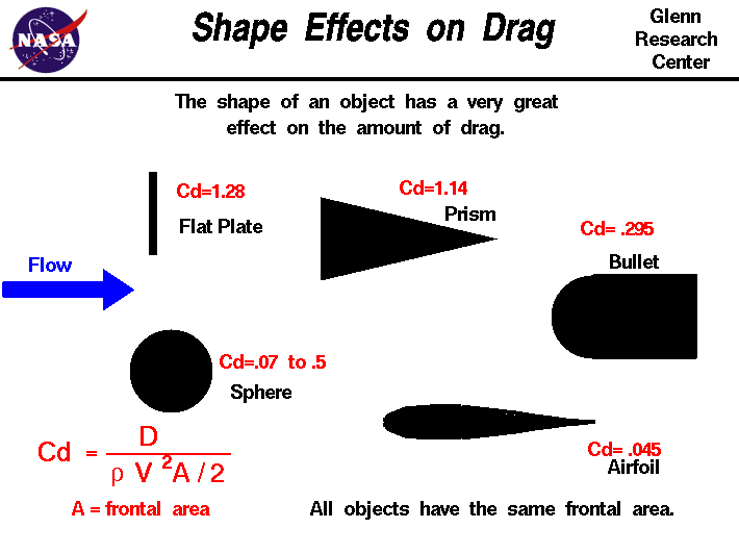
\includegraphics[width=0.7\linewidth]{shapedrag}
	\caption{Shape effect on drag}
\end{figure}

Regarding the lift coefficient a strong simplification as made. For a flat plate the lift coefficient can be approximated with the following formula based on the angle of attack\footnote{\url{http://brennen.caltech.edu/fluidbook/externalflows/lift/flatplateairfoil.pdf}} :
\begin{equation}
	C_L = 2\pi\sin(\alpha)
\end{equation}

For an angle of attack of $11^\circ$ the result for the lift coefficient is $1.2$.\\

To reduce fuel consumption for attitude control a constant angle of attack would be beneficial. To achieve this, the angle between the resulting vector of lift and drag and the velocity vector needs to be the same as the angle between the resulting vector of decelerating and inclination changing vector and the velocity vector. The required delta-Vs for decelerating and inclination change are perpendicular to each other and the angle between them is given by:

\begin{align}
	\beta_{\Delta v_{res}}&=\arctan\bigg(\frac{\Delta v_{inc_{2_p}}}{\Delta v_5}\bigg) = 76^\circ\\
	\beta_{F_{res}} &= \arctan\bigg(\frac{C_L}{C_D}\bigg)
\end{align}

To compute the angle of attack these formulas need to be equated and the formula for $C_L$ included.\\

\begin{equation}
	\alpha = \arcsin(\frac{\Delta v_{inc2_p}}{\Delta v_5}\times \frac{C_D}{2\pi})
\end{equation}

For an angle of attack of $11^\circ$ the angle of the resulting vector of lift and drag is $76^\circ$. This results in a balance of both forces during each aerobrake.\\

To estimate the altitude of the aerobrakes, the Matlab function atmoscoesa was used. Here the density of the atmosphere is calculated by altitude between $0$ and roughly $84000$ m. The values for higher altitudes are extrapolated. A higher altitude results in a longer necessary time in the atmosphere. This has the benefit of a slower heating up of the spacecraft and low values for lift and drag forces. However this could require a higher number of aerobrakes. Weighing these parameters against each other an altitude of $82$ km was chosen for the aerobrakes. At this altitude the total aerobraking time is $30.4$ minutes. At a number of $20$ aerobrakes each would take roughly 91 seconds. During the first aerobrake the distance traveled would be roughly $937$ km and during the last roughly $730$ km. The forces acted upon the spacecraft are $13.9$ kN for lift and $3.5$ kN for drag. At a remaining scpacecraft mass of $3000$ kg this adds up to an acceleration of $4.8$ km/s$^2$ so roughly $0.5$ Gs. These values seemed reasonable since this would keep the mechanical stress relatively low allowing for reusability of the GREDER spacecraft.\\

Regarding the thermal loads on the spacecraft the heat shield needs a little more detail. Modeling the heat flux and conductance within the heat shield is simplified due to complexity. Since the even distribution of the heat over the shield is inaccurate several conservative assumptions shall leave a margin for this. CFRC retains its mechanical properties up to $2400^\circ$ C\footnote{\url{https://www.makeitfrom.com/material-properties/Carbon-Carbon}}. The maximum allowable temperature used for the heat shield modeling is 2000 Kelvin. Also, the assumed temperature at the beginning of the aerorakes is $400$ Kelvin. Furthermore It is assumed that the entire kinetic energy is converted to thermal energy and this is completely distributed onto the spacecraft. In reality however not only the spacecraft but also the atmosphere would be heated through friction. This is highly dependent on the geometry of the body. Most reentry vehicles use blunt front faces to "push" a protective shock wave heat shield in front of them. This keeps the highest heat loads away from the surface. This affect can be seen in \autoref{figtim1} below. \\
\begin{figure}[H]
	\centering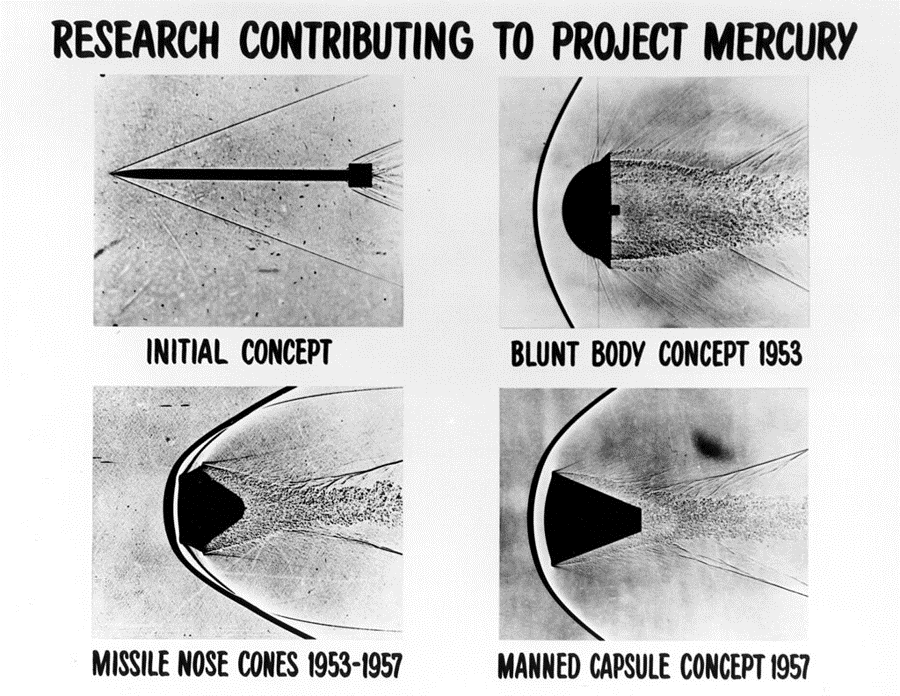
\includegraphics[width=\linewidth]{shadowgraph}
	\caption{Shadowgraph images of Reentry vehicles}\label{figtim1}
\end{figure}

As a further simplification, heat transfer is considered solely through convection during the aerobrake maneuver and solely through radiation during the completion of each orbit. The short duration of the aerobrakes is not very significant compared to the duration of a completed orbit ($90$ s vs. roughly $90$ minutes). Furthermore the heat capacity of CFRC increases with increasing temperature. At $750$ Kelvin the specific heat capacity is roughly double the value compared to ambient temperature (Specific Heat of Carbon/Carbon Composites \footnote{\url{https://apps.dtic.mil/dtic/tr/fulltext/u2/a106709.pdf }}) This leaves an increased margin during the peak heat loads of the atmospheric breaking.\\

To avoid mechanical failure of the spacecraft hull beneath the heat shield a aerogel layer is introduced due to its excellent isolating properties and very low density. Here a $10$ mm layer of silica aerogel blankets at a density of roughly $20$0 kg/m$^3$ is utilized. \\

The thermal loads are expected to be highest on the leading edges of the spacecraft's wings and the nose of the spacecraft. In these areas the heat shield shall have the largest thickness. \autoref{figtim1} shows the areas where the heat shield will be applied. roughly half of the GREDER spacecraft will be covered by the heat shield. This includes the lower faces and leading faces. The upper side and rear of the spacecraft is not expected to endure high thermal loads during the aerobraking maneuvers since the nose will be tilted upwards exposing the lower side.\\

\textbf{Final heat shield mass} : 
\begin{align}
	m_{shield_cc} &= \frac{m_{sc} \times (\Delta v_5\times 1000)^2}{40\times c_{cc}(T_{max_{cc}}-T_0)} = 344.9\ kg\\
	m_{aerogel} &= A_v\times 0.01\times 200 = 17.3kg\\
	m_{shield_{total}} &= 362.2 kg
\end{align}
\begin{figure}[H]
	\centering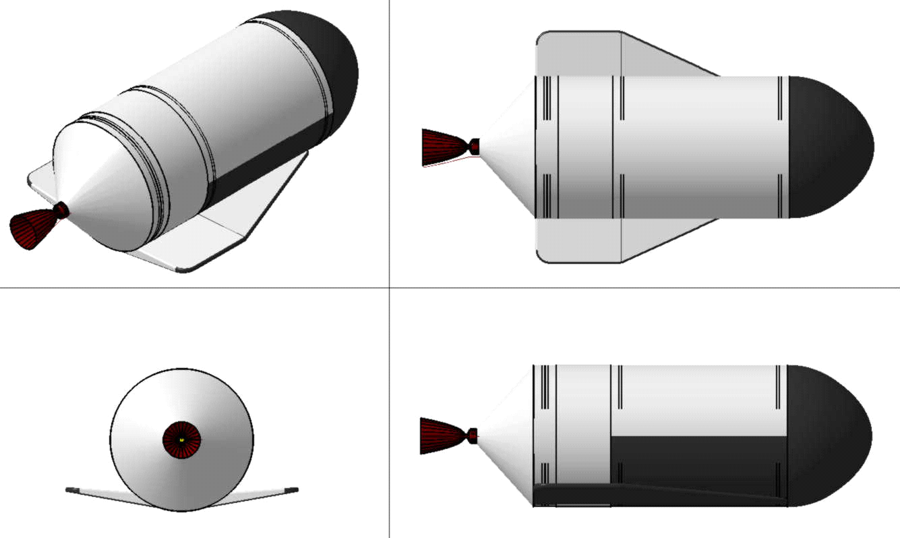
\includegraphics[width=\linewidth]{grederviews}
	\caption{GREDER Spacecraft (various views) - Heat shield sown in gray}
\end{figure}